\documentclass[a4paper]{article}

%% Language and font encodings
\usepackage[spanish]{babel}
\usepackage[utf8]{inputenc}
\usepackage[T1]{fontenc}


%% Sets page size and margins
\usepackage[a4paper,top=3cm,bottom=2cm,left=3cm,right=3cm,marginparwidth=1.75cm]{geometry}

%% Useful packages
\usepackage[utf8]{inputenc}
\usepackage[spanish]{babel}
\usepackage{hyperref}
\usepackage{graphicx}
\usepackage{wrapfig}
\usepackage[square,numbers]{natbib}
\usepackage{amsmath}
\usepackage{float}
\usepackage{xcolor}


\title{Fast and Efficient Method for
Fire Detection Using Image Processing}
\author{Bianca Bramati y Joaquín Laks}
\date{}

\begin{document}
\maketitle

\section{Introduction}
\textcolor{red}{falta hacer}

\section{Metolodología}

\subsection{Análisis de color}
El primer paso del método trabaja sobre cada frame del video independientemente. Consiste en realizar un análisis del escena teniendo en cuenta solamente sus colores. Utilizamos el modelo de color \textbf{CIE L*a*b*}.

Este modelo consiste en representar cada píxel con tres componentes:
\begin{itemize}
    \item $L$* representa la \textbf{luminosidad} del píxel.
    \item $a$* representa la presencia de \textbf{verde-rojo} (valores negativos hacia verde, valores positivos hacia rojo).
    \item $b$*, la presencia de \textbf{azul-amarillo} (valores negativos hacia azul, valores positivos hacia amarillo).
\end{itemize}

\begin{figure}[H]
    \centering    
    \fbox{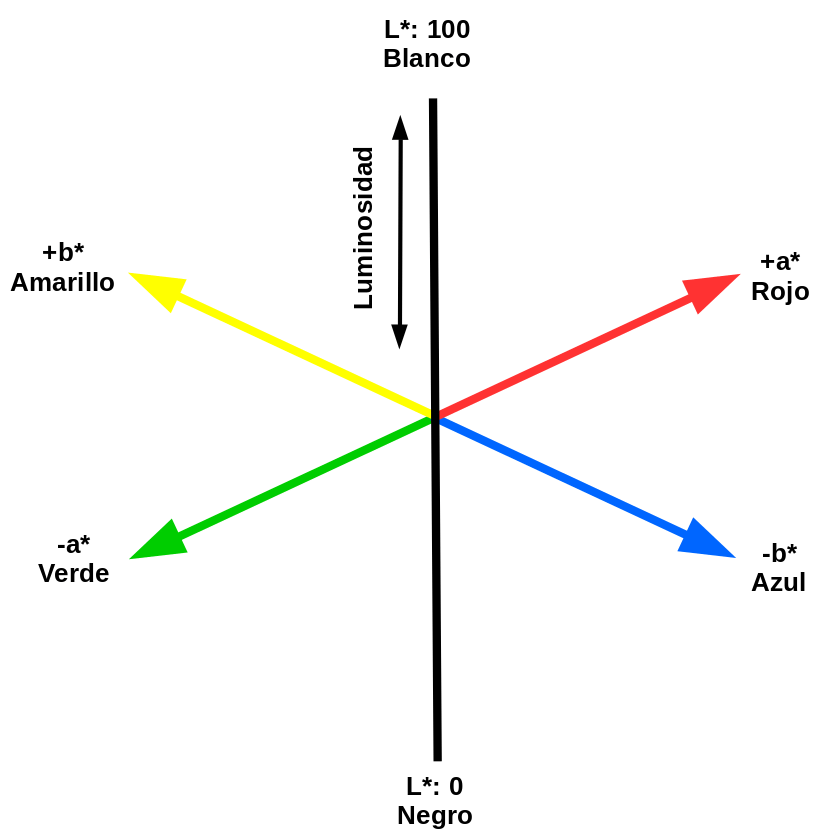
\includegraphics[width=0.28\linewidth]{figures/cie_lab.png}}
\end{figure}

En base a este modelo de color, se definen los valores $L^*_m$, $a^*_m$ y $b^*_m$, siendo cada uno de ellos el valor promedio de dicha componente en la imagen. A partir de estos promedios, calculamos las máscaras $R_1, R_2, R_3, R_4$, con la intención de definir un espacio de color posible para el fuego:

\[
R_1(x,y) = 
\begin{cases}
    1, & \text{si } L^*(x,y) \geq L^*_m, \\
    0, & \text{caso contrario,}
\end{cases}
\]

\[
R_2(x,y) = 
\begin{cases}
    1, & \text{si } a^*(x,y) \geq a^*_m, \\
    0, & \text{caso contrario,}
\end{cases}
\]

\[
R_3(x,y) = 
\begin{cases}
    1, & \text{si } b^*(x,y) \geq b^*_m, \\
    0, & \text{caso contrario,}
\end{cases}
\]

\[
R_4(x,y) = 
\begin{cases}
    1, & \text{si } b^*(x,y) \geq a^*(x,y), \\
    0, & \text{caso contrario,}
\end{cases}
\]

Definimos, además, $P\big(L^*(x,y), a^*(x,y), b^*(x,y)\big)$, como la probabilidad que $L^*$, $a^*$, $b^*$ pertenezcan a una región de fuego. Se calcula para cualquier valor de $L^*$, $a^*$ y $b^*$ en base a un análisis con imágenes previamente segmentadas y etiquetadas. Usando este concepto, definimos una última máscara $R_5$, que mantiene pixeles con mayor probabilidad de pertenecer a una región de fuego: 

\[
R_5(x,y) = 
\begin{cases}
    1, & \text{si } P\big(L^*(x,y), a^*(x,y), b^*(x,y)\big) \geq \alpha, \\
    0, & \text{caso contrario,}
\end{cases}
\]

siendo $\alpha$ es un threshold.

Luego, la máscara final, $F$, mantiene aquellos píxeles que han sido mantenidos por $R_1, R_2, R_3, R_4$ y $R_5$:
\[
F(x,y) =
\begin{cases}
1 & \text{if } \sum_{i=1}^5 R_i(x,y) = 5, \\
0 & \text{caso contrario}.
\end{cases}
\]

Solo este procedimiento no alcanzaría para detectar fuego con certeza, habiendo una gran variedad de objetos rojos que no son fuego e igual se detectarían de esta forma. 

\subsection{Análisis de movimiento de pixeles}
Como segundo paso, se sigue la idea que los píxeles pertenecientes a una región de fuego presentarán cambios (movimiento) entre frames consecutivos. 

Para determinar si un píxel $(x,y)$ está en movimiento en un instante $t$, generamos dos máscaras binarias para cada frame: \textbf{Foreground Difference} (FD), y \textbf{Background Difference} (BD).

\[
FD(x,y,t) = 
\begin{cases}
    1, & \text{si } \left| L^*(x,y,t) - L^*(x,y,t-1) \right| \geq T_{FD}, \\
    0, & \text{caso contrario,}
\end{cases}
\]

\[
BD(x,y,t) = 
\begin{cases}
    1, & \text{si } \left| L^*(x,y,t) - BG(x,y,t-1) \right| \geq T_{BD}, \\
    0, & \text{caso contrario,}
\end{cases}
\]

donde $BG(x,y,t-1)$ es la luminosidad del fondo de la imagen en el instante $t-1$, obtenida analizando valores estáticos del frame previo. Los thresholds $T_{FD}$ y $T_{BD}$ se calculan de forma dinámica para cada frame:
\begin{itemize}
    \item $T_{FD}$ es la suma de la media $\mu$ y la desviación estándar $\sigma$ de $\left| L^*(x,y,t) - L^*(x,y,t-1) \right|$ para el frame del tiempo $t$.

    \item $T_{BD}$ es la suma de la media $\mu$ y la desviación estándar $\sigma$ de $\left| L^*(x,y,t) - BG(x,y,t-1) \right|$ para el frame del tiempo $t$.
\end{itemize}

Con estas dos máscaras, definimos la matriz de movimiento:
\begin{align*}
    M(x,y) = FD(x,y,t) \oplus BD(x,y,t)
\end{align*}

Es decir, consideramos que un píxel está en movimiento si $FD(x,y,t) = 1$ ó $BD(x,y,t) = 1$. 

Juntando el análisis de color y de movimiento, un píxel ''candidato'' a ser parte de una región de fuego cumple:
\begin{align*}
    CF(x,y,t) = F(x,y) \otimes M(x,y)
\end{align*}

\subsection{Análisis de componentes conexas}
Como último paso, se analizan las \textbf{componentes conexas} de los píxeles $(x,y)$ que cumplen $CF(x,y,t)$.

La motivación es que, en sus etapas tempranas, el fuego suele crecer espacialmente, por ende el número de píxeles detectados en una región de fuego debería incrementar. Entonces, se tienen en cuenta componentes conexas que crecieron en área en los últimos frames.

Llamamos $O(t)$ a la componente conexa a analizar en el instante de tiempo $t$, y $NO(t)$ la cantidad de píxeles en $O(t)$. Definimos contador $CGO(t)$, que aumentará respecto al instante $t-1$ si en $t$ aumenta la cantidad de píxeles. Se actualiza como:
\[
CGO(t) =
    \begin{cases}
        CGO(t-1) + 1, & \text{si } NO(t) \geq NO(t-1) \\
        CGO(t-1), & \text{caso contrario.}
    \end{cases}
\]
 

\section{Evaluación}
Dados estos tres pasos, consideramos que el algoritmo detectó fuego si luego de aplicarlos a un frame, aún tenemos píxeles de valor mayor a cero.

Realizamos la evaluación del método de dos formas:

Primero, comparamos solamente el resultado del análisis de color, con una segmentación realizada por el algoritmo de Otsu sobre la componente $a^*$. 

Este es un método para segmentar imágenes, propuesto por Nobuyuki Otsu$^2$. En su versión más simple, separa la imagen en dos clases, y calcula un threshold que clasifica los píxeles en alguna de ellas. El threshold se calcula minimizando la varianza entre los píxeles de cada clase.

Luego, evaluamos el método completo con videos, comparando para cada frame estas tres opciones:
\begin{itemize}
    \item El método original, es decir, $R_1, \dots, R_5$.
    \item Otsu sobre la componente $a^*$.
    \item Otsu sobre la componente $a^*$ combinado con $R_5$.
\end{itemize}
  
 
 
\section{Resultados}
\textcolor{red}{falta escribir un poco. Las tablitas tendría que rehacerlas pero no me dio el tiempo}

 
\begin{figure}[H]
    \centering
    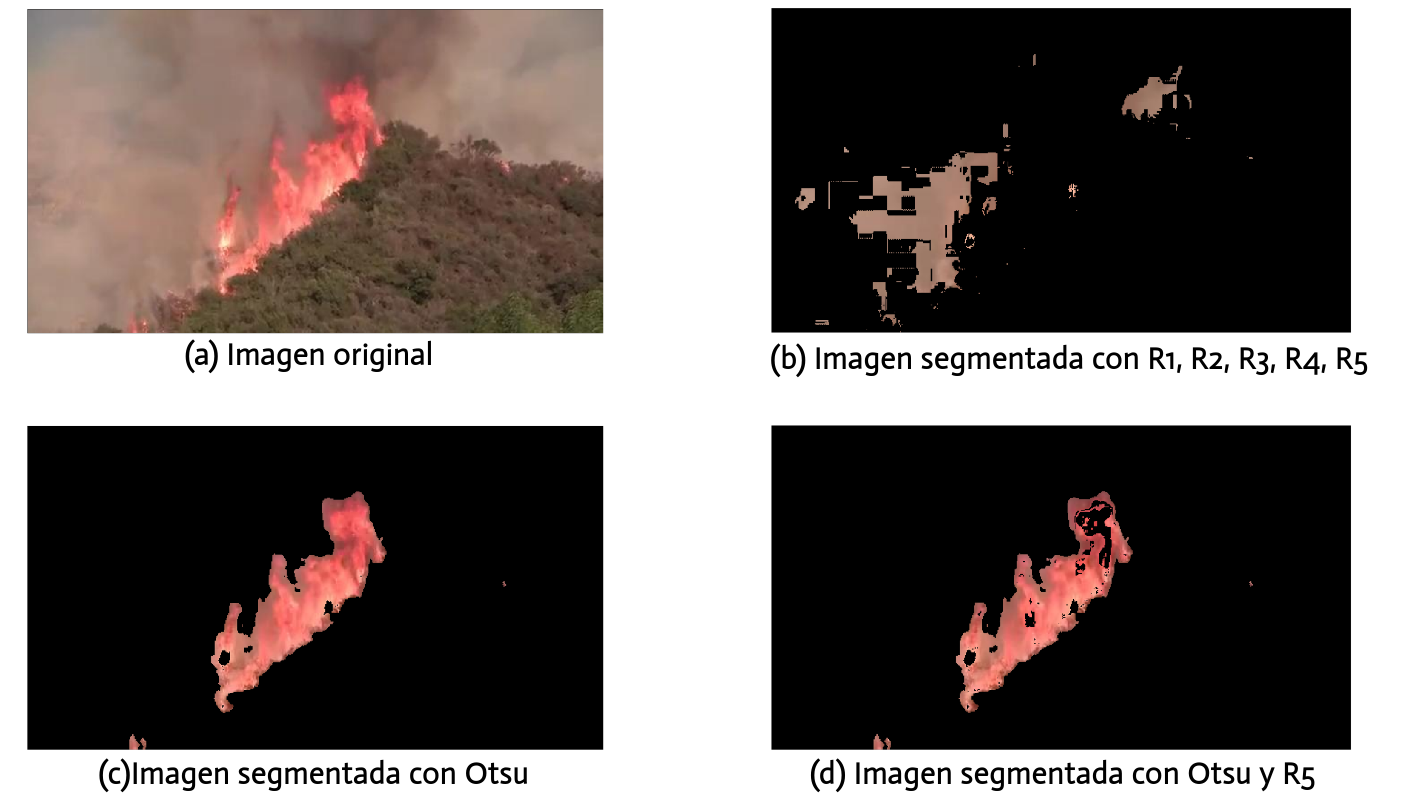
\includegraphics[width=1\linewidth]{figures/exp_img.png}
\end{figure}

\begin{figure}[H]
    \centering
    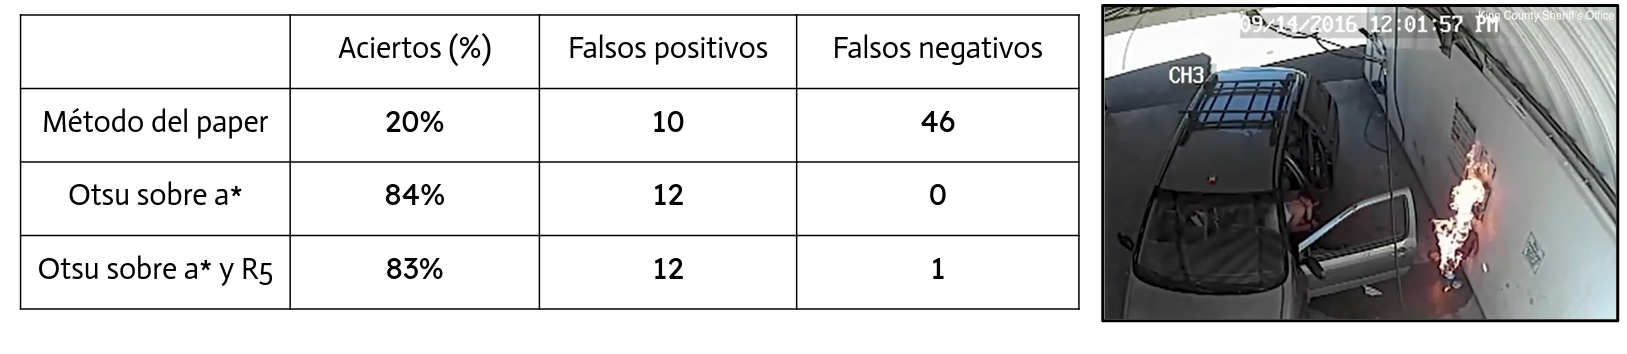
\includegraphics[width=1\linewidth]{figures/exp_video_1.png}
    \label{fig:exp_video_1}
\end{figure}
 

\begin{figure}[H]
    \centering
    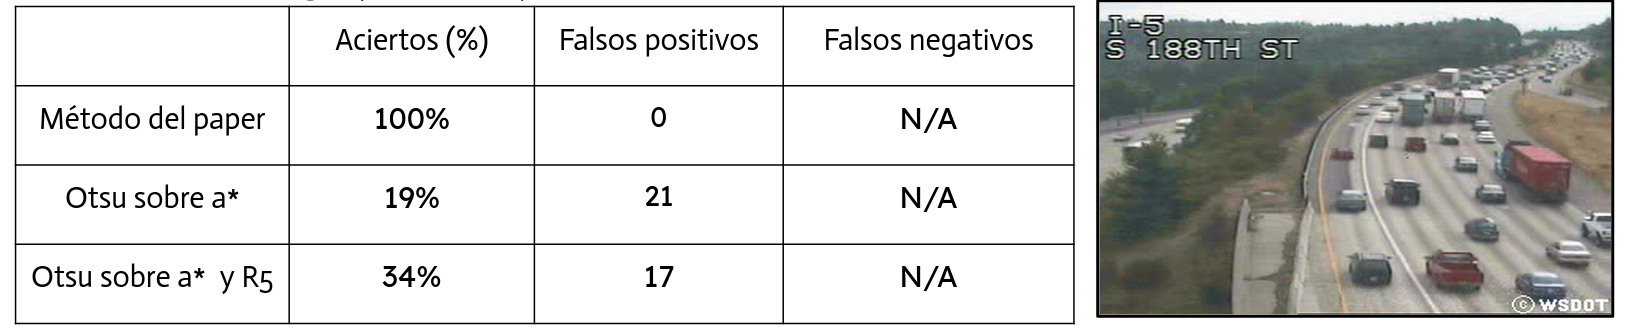
\includegraphics[width=1\linewidth]{figures/exp_video_2.png}
\end{figure}
 

\begin{figure}[H]
    \centering
    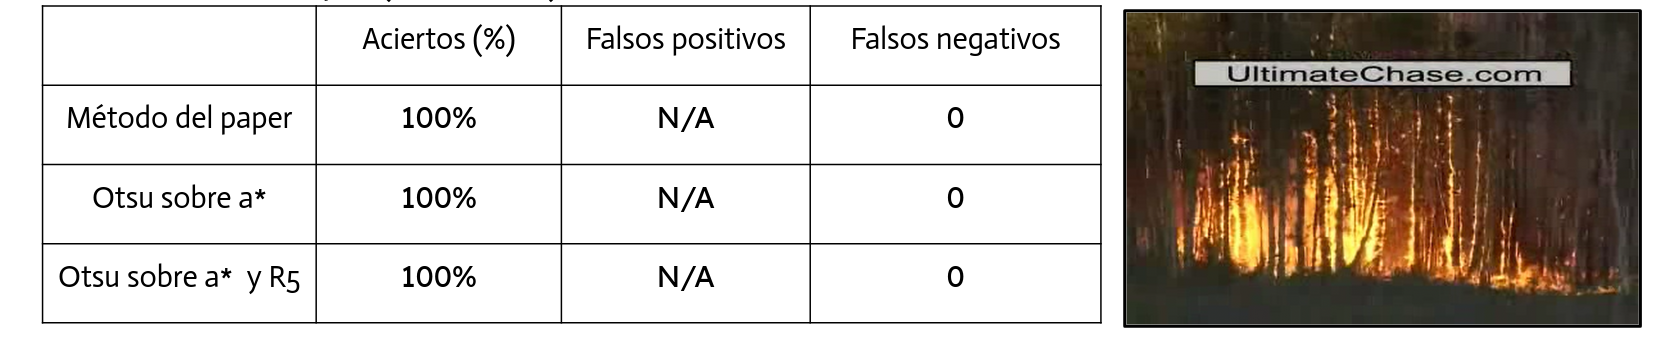
\includegraphics[width=1\linewidth]{figures/exp_video_3.png}
    \label{fig:exp_video_3}
\end{figure}
 

\begin{figure}[H]
    \centering
    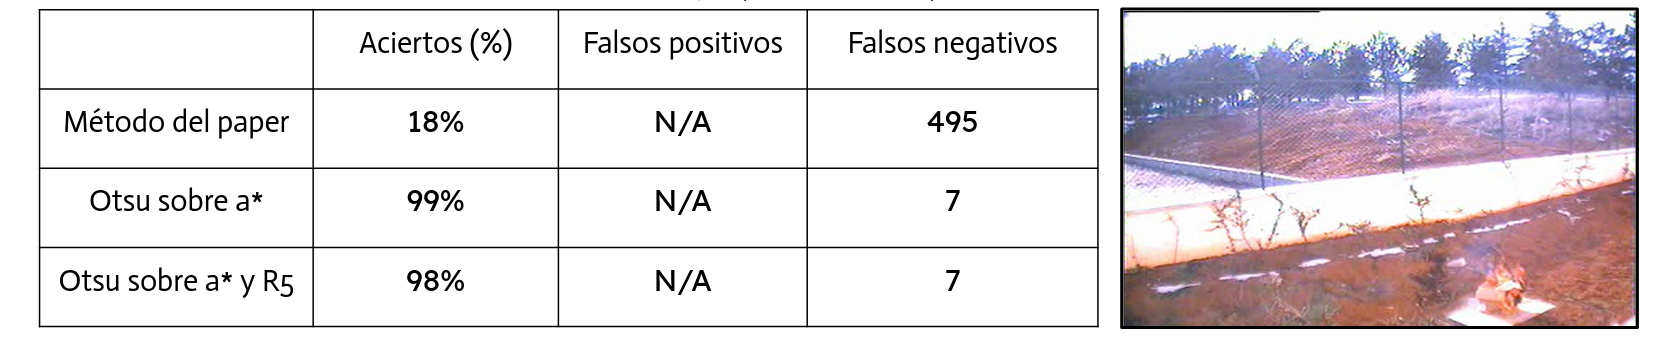
\includegraphics[width=1\linewidth]{figures/exp_video_4.png}
    \label{fig:exp_video_4}
\end{figure}
 



\section{Conclusión}
\textcolor{red}{falta hacer}

\bibliographystyle{abbrvnat}
\begin{thebibliography}{9}
\bibitem{paper} 
Celik, T. (2010).
\textit{Fast and efficient method for fire detection using image processing.} ETRI journal, 32(6), 881-890.

\bibitem{otsu} 
Otsu, N. (1975)
\textit{A threshold selection method from gray-level histograms}. Automatica, 11(285-296), 23-27. 

\bibitem{dataset} 
A. E. Çetin (2014) 
\textit{Computer Vision Based Fire Detection Dataset.}

\end{thebibliography}
\end{document}